\chapter{Implementazione}

\section{Descrizione del progetto}

\todo{Una descrizione del progetto, con la separazione in fasi}

%%%% STRUMENTI %%%%%
\section{Strumenti}

I dati che sono stati analizzati in questo progetto di tesi sono stati scaricati
dal database di Scopus utilizzando le API che il sito mette a disposizione.

Per implementare la dashboard e le varie pagine che mostrano i risultati delle
interrogazioni è utilizzato Python come linguaggio di programmazione, il
framework Django e SQLite come database.

%%%% SCOPUS API %%%%%
\subsection{Scopus API}

Scopus permette di accedere a circa 78 milioni di articoli, riviste
scientifiche, libri e pubblicazioni. Le API di Scopus permettono di visualizzare
abstract e dati riguardanti il numero di citazioni di tutte le riviste
accademiche indicizzate da Scopus.

Sono disponibili due modi di utilizzo delle API di Scopus: commerciale e
non commerciale. Per questa tesi sono state utilizzate le API a uso non
commerciale, disponibili gratuitamente per lavori senza scopo di lucro.
Utilizzando le API di Scopus si ha accesso diretto ai dati di Scopus in tempo
reale. Le \textit{API responses} includono link a risorse collegate, rendendo
la navigazione più semplice e la documentazione consente di visualizzare in
anteprima la richiesta e la risposta della API in modo interattivo. Inoltre
l'architettura RESTful permette di avere vantaggi di scalabilità, portabilità
e affidabilità.
Tali API risultano però sottoposte ad alcuni limiti, in quanto sono accessibili
solo da reti di atenei riconosciute da Scopus ed implementano rate limiting\footnote{\url{https://dev.elsevier.com/api_key_settings.html}}.

Una categoria di API importante è rappresentata dalla \textit{Scopus Search}~\cite{scopussearch}.
Essa può essere usata per accedere a dati riguardanti
paper, con relativi autori ed atenei. Ogni risultato fornito è collegato ad un
abstract e tramite link al resto del testo dell'articolo.
Questa API utilizza la sintassi booleana che consente agli utenti di combinare
parole chiave attraverso gli operatori \texttt{AND}, \texttt{OR} e \texttt{NOT},
per poter produrre risultati  più rilevanti. La ricerca booleana viene inviata
tramite il parametro \textit{query} della \textit{query string} e il contenuto
della ricerca inviata deve essere  codificato nell'URL.

\subsection{pybliometrics}\label{sec:pybliometrics}

\texttt{pybliometrics}~\cite{pybliometrics} è una libreria di Python che serve per estrarre e
memorizzare nella cache i dati dal database Scopus.
Essa fornisce un insieme di classi che forniscono un'astrazione dalle chiamate
API di Scopus. Tali classi sono:
\begin{itemize}
	\item \texttt{AbstractRetrieval}: implementa l'API Abstract Retrieval di
	Scopus che consente di estrarre informazioni riguardo gli articoli;
	\item \texttt{AffiliationRetrieval}: implementa l'API Affiliation Retrieval
	di Scopus che fornisce informazioni riguardo gli atenei registrati, come per
	esempio città, paese e membri;
	\item \texttt{AuthorRetrieval}: implementa l'API Author Retrieval di Scopus
	che contiene tutte le informazioni riguardanti un autore;
	\item \texttt{ScopusSearch} implementa l'API di ricerca di Scopus, esegue una
	query per cercare documenti e quindi recupera i record della query.
  \end {itemize}

%%%% DJANGO %%%%%
\subsection{Django}

Django~\cite{django} è un framework web open source scritto in Python. È
un framework ``batteries included'', ovvero tenta di fornire più strumenti
possibile per ridurre sia la quantità di codice da scrivere sia la sua
complessità.

Django si basa sull'architettura \textit{Model, View, Template}, basata sulla più
classica MVC. Essa propone tre diverse entità per la gestione dei dati e dell'interazione
con l'utente, che sono:
\begin{itemize}
	\item \textit{Model}, la descrizione dei dati tramite una classe Python;
	\item \textit{View}, un sistema che processa le richieste degli utenti e
	definisce che dati devono essere presentati in risposta;
	\item \textit{Template}, un template HTML con un proprio linguaggio di templating
	chiamato DTL (Django Template Language) che definisce la rappresentazione
	grafica dei dati.
\end{itemize}
In questa categorizzazione, la \textit{View} di MVT corrisponde al \textit{Controller}
di MVC, mentre il \textit{Template} di MVT corrisponde alla \textit{View} di MVC.

\begin{lstlisting}[language=Python,caption=La classe \texttt{Author},       label=lst:author]
from django.db import models

class Author(models.Model):
    surname = models.CharField(max_length=200)
    name = models.CharField(max_length=200)
    citation_count = models.IntegerField()
    cited_by_count = models.IntegerField()
    h_index = models.IntegerField()
\end{lstlisting}

Django fornisce un ORM (\textit{Object-Relational Mapping}) tramite la
rappresentazione di tabelle con delle classi che derivano dalla classe
predefinita \texttt{Model}, come mostrato nel Listing~\ref{lst:author}. In
tal modo, è possibile interagire con degli oggetti Python, del tutto simili
alle classi, astraendo completamente dalla tecnologia di database utilizzata.
Infatti, con Django è possibile utilizzare diversi DBMS~\cite{djangoDBMS}, tra cui PostgreSQL,
MariaDB, MySQL e SQLite. Quest'ultimo è stato scelto per essere usato in questo
progetto di tesi, in quanto la semplicità e la facilità di setup sono risultate
fondamentali per velocizzare la realizzazione di prototipi.

Le \textit{View} di Django possono essere rappresentate da varie entità nel codice,
ma i modi principali sono le \textit{view generiche} tramite classi fornite dal framework
stesso e delle semplici \textit{funzioni} che lavorano su un parametro rappresentante
la richiesta effettuata dall'utente. Come esempio, nel Listing~\ref{lst:view-author-info}
è rappresentata una view che ottiene le informazioni di un autore specifico,
come salvate su database, aggiungendo inoltre una classificazione in base al
rating delle conferenze a cui ha partecipato.

\begin{lstlisting}[language=Python,caption=La view \texttt{author\_info},label=lst:view-author-info]
def author_info(request, author_id):
    author = get_object_or_404(Author, pk=author_id)
    num_confs = {}

    for pub in author.publication_set.all():
        rating = pub.paper.conference.ggs_rating
        if rating in num_confs:
            num_confs[rating] += 1
        else:
            num_confs[rating] = 1

    return render(request,
                  "author_info.html",
                  {"author": author, "num_confs": num_confs})
\end{lstlisting}

\section{Ottenimento dei dati}

Come già anticipato in Sezione~\ref{sec:scopus}, la maggior parte dei dati è
stata presa da Scopus. In particolare, Scopus ha fornito i dati di circa 80000
papers negli ultimi 4 anni, con i relativi autori ed affiliazioni.
Per le conferenze, non fornendo Scopus informazioni se non nome ed acronimo
delle conferenze, si è fatto uso dei dati indicizzati da GII-GRIN-SCIE~\cite{giigrinscie} (GGS).

Per il download dei dati da Scopus, si è usato \texttt{pybliometrics}
(Sezione~\ref{sec:pybliometrics}) per lo sviluppo di script custom orientati
al download di grandi quantità di dati in modo automatico facendo uso delle
API fornite da Scopus.

Per quanto riguarda le conferenze, invece, i nomi delle conferenze forniti da
GGS non concordano in pieno con quelli presenti su Scopus. A questo fine,
si è manualmente proceduto all'analisi delle conferenze ottenute ed al loro
inserimento all'interno del database del progetto.
Al fine di semplificare e velocizzare il processo, si è fatto uso della
\textit{distanza di Levenshtein} per confrontare i nomi dati dalle due fonti.
La priorità è stata comunque data agli acronimi rispetto ai nomi interi.

\subsection{Distanza di Levenshtein}

L'algoritmo di Levenshtein, introdotta per la prima volta nel
1965~\cite{levenshtein1966} calcola la somiglianza tra due stringhe diverse.
Date due stringhe $a$ e $b$, l'algoritmo misura il numero di modifiche
elementari necessarie per trasformare la stringa $a$ nella stringa $b$.
Tra le operazioni elementari si hanno eliminazione di un carattere,
sostituzione di un carattere con un altro, inserimento di un nuovo carattere.
Più precisamente, definite $a$ e $b$ due stringhe, $|a|$ la lunghezza di una
stringa, la distanza di Levenshtein è definita come
\begin{equation*}
  \text{lev}(a, b) =
  \begin{cases}
    |a| & \text{se } |b| = 0 \\
    |b| & \text{se } |a| = 0 \\
    \text{lev}(\text{tail}(a), b) & \text{se } a_0 = b_0 \\
    1 + \min\begin{cases}
      \text{lev}(\text{tail}(a), b) \\
      \text{lev}(a, \text{tail}(b)) \\
      \text{lev}(\text{tail}(a), \text{tail}(b)) \\
    \end{cases}
    & \text{altrimenti}
  \end{cases}
\end{equation*}
%
Dove $\text{tail}$ rappresenta la coda di una lista, i.e., se $a_i$ è il
carattere in posizione $i$, allora data la stringa $a = a_0a_1\cdots a_n$ si ha
che $\text{tail}(a) = a_1\cdots a_n$.
Nell'implementazione è stata usata la libreria
\texttt{python-Levenshtein}~\cite{pythonLevenshtein}.

%%% DOWNOLAD DEI DATI %%%%
\section{Descrizione dei dati}\label{sec:descrizionedati}

In Figura \ref{fig:logico} è visibile lo schema logico, rappresentante
le tabelle presenti direttamente nel database, coi relativi attributi e chiavi
esterne. Notare la presenza della tabella \textit{Publication}, in sostituzione
alla relazione tripla nominata in Sezione~\ref{sec:modellizzazioni}.

Al fine di identificare univocamente i dati, si è fatto uso dei campi
identificativi forniti direttamente dal database di Scopus. Questo per evitare
ambiguità con un'eventuale generazione automatica a partire dai dati,
soprattutto in caso di omonimie.

\begin{figure}
  \centering
  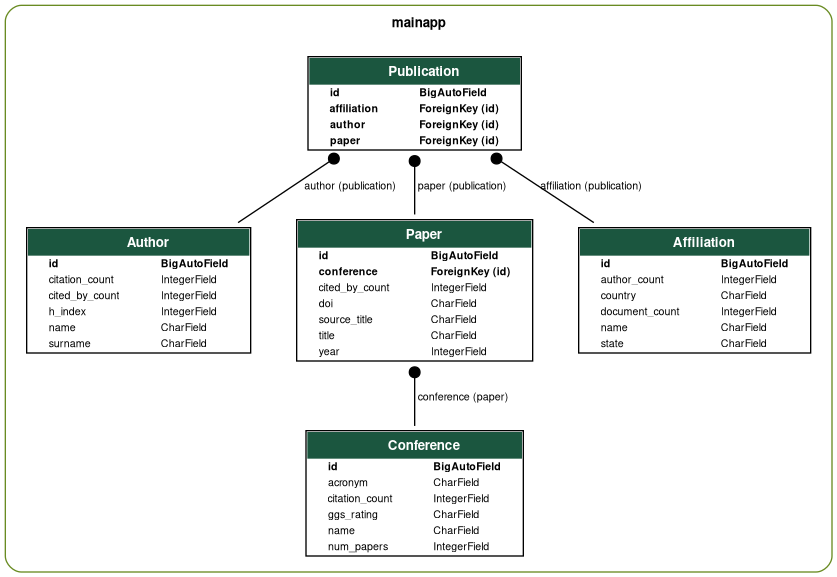
\includegraphics[width=0.8\linewidth]{logico.png}
  \caption{Schema logico del problema}
  \label{fig:logico}
\end{figure}

\subsection{Affiliation}

Un'affiliazione rappresenta un'università, e per ogni singola entry si ha
interesse a mantenere i seguenti campi:

\begin{itemize}
  \item \texttt{aff\_id}, l'identificativo dell'università;
  \item \texttt{affiliation\_name}, nome dell'università;
  \item \texttt{state} e \texttt{country}, contenenti informazioni riguardanti la posizione geografica dell'università;
  \item \texttt{author\_count}, numero di autori associati all'università;
  \item \texttt{document\_count}, numero di documenti per l'università.
\end{itemize}

\subsection{Author}
Un autore è rappresentato dai seguenti campi:
\begin{itemize}
  \item \texttt{author\_id};
  \item dati per il nominativo, ovvero \texttt{surname} e \texttt{name};
  \item \texttt{citation\_count}, numero totale di elementi citati;
  \item \texttt{cited\_by\_count}, numero totale di autori citanti;
  \item \texttt{h\_index}, h-index dell'autore.
\end{itemize}

\subsection{Conference}

Di una conferenza ci interessa mantenere i seguenti campi:
\begin{itemize}
  \item \texttt{title}, nome della conferenza;
  \item \texttt{acronym};
  \item \texttt{ggs\_rating}, il rate come definito da GGS;
  \item \texttt{num\_papers}, numero di paper accettati dalla conferenza;
  \item \texttt{citation\_count}, numero di citazioni totali di tutti i paper della conferenza.
\end{itemize}

\subsection{Paper}

Un paper viene rappresentato dai seguenti dati:

\begin{itemize}
  \item \texttt{id};
  \item \texttt{authors}, lista di autori del paper (rappresentati dai relativi identificativi);
  \item \texttt{title};
  \item \texttt{year};
  \item \texttt{conference}, la conferenza a cui è stato presentato;
  \item \texttt{cited\_by\_count}, il numero di citazioni;
  \item \texttt{doi}, il suo identificativo DOI.
\end{itemize}

% \section{Implementazione di views e metriche}


